\section{Representation of partitioned transmembrane current}\label{part}
Further progress requires expressions for $I_\mathrm{P}$ and
$I_\mathrm{D}$ in terms of the biophysical and morphological
properties of the segment and the membrane potentials at its
proximal and distal boundaries. Each component of the
transmembrane current (\ref{tc2}) is examined separately.

\subsection{Point sources of transmembrane current}
There are two types of point sources of transmembrane current:
point currents depending on transmembrane potential (synaptic
current), often modelled by the constitutive equation
$\mathcal{I}=g(t)(V-E)$ where $E$ is the reversal potential
associated with the synapse and $g(t)$ is the time course of the
synaptic conductance, and those point currents which are
independent of membrane potential (exogenous current).

Suppose that $\lambda_1,\ \cdots,\lambda_n$ are sites of
point input $\mathcal{I}_1,\ \cdots\ \mathcal{I}_n$
to the segment, then the expressions for $I_\mathrm{P}$ and
$I_\mathrm{D}$ are
\begin{equation}\label{ei1}
I_\mathrm{P} = \sum_{k=1}^n\,
\frac{r_\mathrm{P}}{r_k}\,(1-\lambda_k)\,\mathcal{I}_k\,,\qquad
-I_\mathrm{D} = \sum_{k=1}^n\,
\frac{r_\mathrm{D}}{r_k}\,\lambda_k\,\mathcal{I}_k
\end{equation}
where $r_k=(1-\lambda_k)\,r_\mathrm{P} +\lambda_k\,r_\mathrm{D}$.
In the special case of exogenous input only,
$\mathcal{I}_k=\mathcal{I}_k(t)$ and expressions (\ref{ei1}) give
the exact partitioning of exogenous point input. When synaptic
input is present, the expressions for $I\mathrm{P}$ and
$I_\mathrm{D}$ will contain the (unknown) membrane potentials at
the synapses. The application of the partitioning rule will
require these potentials to be estimated in terms of known
functions and the potentials at the proximal and distal boundaries
of the segment. One obvious way to do this is to use the potential
distribution (\ref{mp3}). However, the derivation of (\ref{mp3})
assumed that transmembrane current was negligible by comparison
with axial current, thus its efficacy in estimating the potential
at a synapse relies on the validity of that assumption. It will be
shown in Subsection \ref{single} that the use of formula
(\ref{mp3}) for a single synapse overestimates the influence of
that synapse. This observation suggests that the partitioning rule
needs to be generalised to include situations in which point input
current is not small by comparison with axial current.

\subsection{Generalisation of partitioning rule for point input}
The partitioning rule may be generalised  by recognising that the
partitioning of transmembrane current does not have to be between
axial currents at the proximal and distal boundaries of the
segment, but may be applied to nearest neighbour sites of a point
input, although, of course, the proximal and distal boundaries of
the segment may be nearest neighbours to one of these sites. This
application of the partitioning rule is equivalent to considering
the balance between axial current and point current at each input
site ignoring the presence of distributed current between sites.
Figure \ref{synapses} is a schematic representation of a segment
of length $h$ illustrating the relative locations $\lambda_1,\
\cdots, \lambda_n$ of $n$ point inputs $\mathcal{I}_1,\ \cdots\
\mathcal{I}_n$ on a segment. Suppose axial current $I_k$ flows to
the point $\lambda_k$ from the point $\lambda_{k-1}$ and that
$V_k$ is the potential at the point $\lambda_k$.

\begin{figure}[!h]
\centering
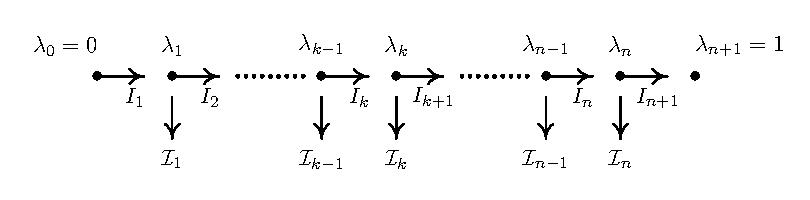
\includegraphics[ ]{NewCompFig3.eps}
\parbox{4in}{\caption{\label{synapses} Configuration of
point input to a dendritic segment of length $h$. Here
$\mathcal{I}_k=g_k(t)(V_k-E_k)$ in the case of a synapse at
$\lambda_k$ or $\mathcal{I}_k=\mathcal{I}_k(t)$ in the case of an
exogenous input.}}
\end{figure}

%\begin{figure}[!h]
%\centerline{\qquad\begin{mfpic}[0.9][1]{-50}{400}{-30}{50}
%\pen{1pt}
%\headlen7pt
%%
%% Sealed cable
%\arrow\lines{(0,20),(25,20)}
%\arrow\lines{(40,20),(65,20)}
%\arrow\lines{(120,20),(145,20)}
%\arrow\lines{(160,20),(185,20)}
%\arrow\lines{(240,20),(265,20)}
%\arrow\lines{(280,20),(305,20)}
%%
%%
%\dotspace=4pt
%\dotsize=2pt
%\dotted\lines{(75,20),(110,20)}
%\dotted\lines{(195,20),(230,20)}
%%
%% Nodes on sealed cable
%\tlabel[cc](0,20){\large $\bullet$}
%\tlabel[cc](40,20){\large $\bullet$}
%\tlabel[cc](120,20){\large $\bullet$}
%\tlabel[cc](160,20){\large $\bullet$}
%\tlabel[cc](240,20){\large $\bullet$}
%\tlabel[cc](280,20){\large $\bullet$}
%\tlabel[cc](320,20){\large $\bullet$}
%%
%% Points on sealed cable
%\tlabel[br](0,30){$\lambda_0=0$}
%\tlabel[bc](40,30){$\lambda_1$}
%\tlabel[bc](120,30){$\lambda_{k-1}$}
%\tlabel[bc](160,30){$\lambda_k$}
%\tlabel[bc](240,30){$\lambda_{n-1}$}
%\tlabel[bc](280,30){$\lambda_n$}
%\tlabel[bl](320,30){$\lambda_{n+1}=1$}
%%
%\tlabel[cc](20,10){$I_1$}
%\tlabel[cc](60,10){$I_2$}
%\tlabel[cc](140,10){$I_k$}
%\tlabel[cc](180,10){$I_{k+1}$}
%\tlabel[cc](260,10){$I_n$}
%\tlabel[cc](300,10){$I_{n+1}$}
%%
%% Sealed cable
%\arrow\lines{(40,10),(40,-10)}
%\tlabel[tc](40,-15){\textsf{$\mathcal{I}_1$}}
%\arrow\lines{(120,10),(120,-10)}
%\tlabel[tc](120,-15){\textsf{$\mathcal{I}_{k-1}$}}
%\arrow\lines{(160,10),(160,-10)}
%\tlabel[tc](160,-15){\textsf{$\mathcal{I}_k$}}
%\arrow\lines{(240,10),(240,-10)}
%\tlabel[tc](240,-15){\textsf{$\mathcal{I}_{n-1}$}}
%\arrow\lines{(280,10),(280,-10)}
%\tlabel[tc](280,-15){\textsf{$\mathcal{I}_n$}}
%\end{mfpic}}
%\centering
%\parbox{4in}{\caption{\label{synapses} Configuration of
%point input to a dendritic segment of length $h$. Here
%$\mathcal{I}_k=g_k(t)(V_k-E_k)$ in the case of a synapse at
%$\lambda_k$ or $\mathcal{I}_k=\mathcal{I}_k(t)$ in the case of an
%exogenous input.}}
%\end{figure}

The potentials $V_1,\ \cdots\ ,V_n$ at the points $\lambda_1,\
\cdots, \lambda_n$ are related to the currents $I_1,\ \cdots\ ,
I_{n+1}$ by making the appropriate replacements in formula
(\ref{mp2}) to get
\begin{equation}\label{syn2}
I_k = \ds\frac{\pi g_\mathrm{A}r_{k-1}\,r_k}
{h(\lambda_k-\lambda_{k-1})}\,\big(V_{k-1}-V_k\,\big)\,,\qquad
k=1,\cdots,(n+1)
\end{equation}
where it is understood that $\lambda_0=0$, $\lambda_{n+1}=1$,
$r_0=r_\mathrm{P}$, $r_{n+1}=r_\mathrm{D}$, $V_0=V_\mathrm{P}$ and
$V_{n+1}=V_\mathrm{D}$. It follows directly from (\ref{syn2}) that
\begin{equation}\label{syn3}
V_k = V_\mathrm{P} -\frac{h}{\pi g_\mathrm{A}}\,\sum_{j=1}^k \,
\frac{(\lambda_j-\lambda_{j-1})}{r_{j-1}\,r_j}\,I_j \,,\qquad
k=1,\cdots,(n+1)\,.
\end{equation}
If $\lambda_k$ is the point of application of an exogenous input
of strength $\mathcal{I}_k(t)$ then
\begin{equation}\label{syn1b}
I_{k+1}+\mathcal{I}_k(t) = I_k\,.
\end{equation}
On the other hand, if there is a synapse at $\lambda_k$, then
$\mathcal{I}_k=g_k(t)(V_k-E_k)$ and conservation of current
requires that
\begin{equation}\label{syn1a}
I_{k+1}+g_k(V_k-E_k) = I_k\,.
\end{equation}
Formula (\ref{syn3}) for $V_k$ is now used to rewrite equation
(\ref{syn1a}) in terms of axial currents to get
\begin{equation}\label{syn4}
I_k-I_{k+1}+\ds\frac{g_k h}{\pi g_\mathrm{A}}\sum_{j=1}^k
\frac{(\lambda_j-\lambda_{j-1})}{r_{j-1}\,r_j}\,I_j =
-g_kE_k+g_kV_\mathrm{P}\,.
\end{equation}
Thus, the current conservation condition at the points
$\lambda_1,\ \cdots,\ \lambda_n$ gives rise to $n$ equations for
the $(n+1)$ currents $I_1,\ \cdots,\ I_{n+1}$. In order to
complete the system of equations that determine $I_1,\ \cdots,\
I_{n+1}$, it is essential to note that the potentials at the
proximal and distal boundaries of the segment are known, and that
this condition constrains the values of these currents to satisfy
\begin{equation}\label{syn5}
\frac{h}{\pi g_\mathrm{A}}\,\sum_{j=1}^{n+1}
\frac{(\lambda_j-\lambda_{j-1})}{r_{j-1}\,r_j}\,I_j =
V_\mathrm{P}-V_\mathrm{D}\,.
\end{equation}
This condition is obtained from equation (\ref{syn3}) by asserting
that $V_{n+1}=V_\mathrm{D}$. Since it is the perturbations to the
axial currents at the proximal and distal boundaries of the
segment that are sought, and not the currents themselves, it is
convenient to replace $I_k$ in equations (\ref{syn1b}, \ref{syn4}
and \ref{syn5}) by $I_\mathrm{PD}+\widehat{I}_k$ where
$\widehat{I}_k$ is the perturbation to $I_k$. If $\lambda_k$ is
the site of an exogenous input then it follows immediately that
\begin{equation}\label{syn7a}
\widehat{I}_k-\widehat{I}_{k+1}=\mathcal{I}_k(t)\,.
\end{equation}
On the other hand, if $\lambda_k$ is the site of a synapse, then
the identity
\begin{equation}\label{syn6}
\sum_{j=1}^k \,\frac{(\lambda_j-\lambda_{j-1})}{r_{j-1}\,r_j}
=\frac{\lambda_k}{r_\mathrm{P}\,r_k}\,,
\end{equation}
which can be established by induction, can be used to verify that
$\widehat{I}_0, \widehat{I}_1,\ \cdots \,\widehat{I}_{n+1}$
satisfy
\begin{equation}\label{syn7b}
\widehat{I}_k-\widehat{I}_{k+1}+\frac{g_k h}{\pi g_\mathrm{A}}
\sum_{j=1}^k \frac{(\lambda_j-\lambda_{j-1})}{r_{j-1}\,r_j}\,
\widehat{I}_j = \mathcal{I}_k(t)
\end{equation}
where the current $\mathcal{I}_k(t)$ is defined by the formula
\begin{equation}\label{syn7c}
\mathcal{I}_k(t)=g_k(t)\,\Big[\,(1-\lambda_k)\frac{r_\mathrm{P}}{r_k}
\,V_\mathrm{P}+\lambda_k\frac{r_\mathrm{D}}{r_k}\, V_\mathrm{D}
-E_k\,\Big]\,.
\end{equation}
Note that $\mathcal{I}_k(t)$ is precisely the current that would
be expected to flow at the $k^{th}$ synapse if the distribution of
potential along the length of the segment is well described by
expression (\ref{mp3}), that is, the potential distribution on the
assumption that transmembrane current acting on the segment is
negligible compared with axial current. Finally, equation
(\ref{syn5}) simplifies to
\begin{equation}\label{syn7d}
r_\mathrm{P}\,r_\mathrm{D}\,\sum_{j=1}^{n+1}
\frac{(\lambda_j-\lambda_{j-1})}{r_{j-1}\,r_j}\,\widehat{I}_j = 0
\end{equation}
where the constant multiplier $r_\mathrm{P}\,r_\mathrm{D}$ has
been added without loss to make the coefficients of this equation
comparable to those appearing in the first $n$ equations.
Equations (\ref{syn7a},\ref{syn7b} and \ref{syn7d}) may be
represented compactly in matrix notation by
\begin{equation}\label{syn8}
A\,\widehat{I}+GC\,\widehat{I}=\mathcal{I}
\end{equation}
where $\widehat{I}=[\widehat{I}_1,\ \cdots\ ,\widehat{I}_{n+1}
]^\mathrm{T}$ is the $(n+1)$ dimensional column vector of
perturbations in axial current, $\mathcal{I}=[\mathcal{I}_1,\
\cdots\ , \mathcal{I}_n,0\,]^\mathrm{T}$ and $A$ is the
$(n+1)\times(n+1)$ matrix
\begin{equation}\label{syn9}
\left[\begin{array}{ccccccc}
1 & \hskip-9pt-1 &  0 & \cdots & \cdots & 0 \\[5pt]
0 &  1 & \hskip-9pt-1 & \cdots & \cdots & 0 \\[5pt]
0 &  0 &  1 & \cdots & \cdots & 0 \\[5pt]
\cdots & \cdots & \cdots & \cdots & \cdots & \cdots \\[5pt]
0 & 0 & 0 & \cdots & 1 & \hskip-9pt-1 \\[5pt]
\ds\frac{\lambda_1 r_\mathrm{P}r_\mathrm{D}}{r_0 r_1} &
\ds\frac{(\lambda_2-\lambda_1)r_\mathrm{P}r_\mathrm{D}}{r_1 r_2} &
\ds\frac{(\lambda_3-\lambda_2)r_\mathrm{P}r_\mathrm{D}}{r_2 r_3} &
\cdots & \ds\frac{(\lambda_n-\lambda_{n-1})r_\mathrm{P}r_\mathrm{D}}{r_{n-1} r_n} &
\ds\frac{(1-\lambda_n)r_\mathrm{P}r_\mathrm{D}}
{r_n r_{n+1}}
\end{array}\right]\,.
\end{equation}
Briefly, $G$ is an $(n+1)\times(n+1)$ diagonal matrix in which the
$(k,k)$ entry is zero if $\lambda_k$ is the site of an exogenous
input and takes the value $g_k(t)$ if $\lambda_k$ is the site of a
synapse. The $(n+1,n+1)$ entry of $G$ is always zero. The matrix
$C$ is a lower triangular matrix of type $(n+1)\times(n+1)$ in
which all the appropriate entries in the $k^{th}$ column take the
value $(\lambda_k-\lambda_{k-1})/(\pi g_\mathrm{A}r_{k-1}\,r_k)$.

\subsection{Special and general solutions of the point input partitioning equations}
Prior to considering the general solution of equation (\ref{syn8})
it is instructive to examine two special applications; the first
concerns the derivation of the perturbations $I_\mathrm{P}$ and
$I_\mathrm{D}$ in the case of a single synaptic input to a
segment, and the second concerns the derivation of these
perturbations in the presence of exogenous input only.

\subsubsection{Single synaptic input}\label{single}
In the case of a single synaptic input at $\lambda_1$, equations
(\ref{syn8}) become
\begin{equation}\label{syn10}
\Big(1+\frac{\lambda_1 h g_1}{\pi g_\mathrm{A} r_\mathrm{P}
r_1}\Big)\widehat{I}_1-\widehat{I}_2 = \mathcal{I}_1(t)\,,\qquad
\frac{\lambda_1 \widehat{I}_1}{r_\mathrm{P}r_1}
+\frac{(1-\lambda_1) \widehat{I}_2}{r_1r_\mathrm{D}} = 0
\end{equation}
with solutions
\begin{equation}\label{syn11}
I_\mathrm{P}=\widehat{I}_1=\frac{r_\mathrm{P}}{r_1}\,\frac{(1-\lambda_1)\mathcal{I}_1(t)}
{1+\gamma}\,,\qquad
-I_\mathrm{D}=-\widehat{I}_2=\frac{r_\mathrm{D}}{r_1}\,\frac{\lambda_1\mathcal{I}_1(t)}
{1+\gamma}\,,\qquad\gamma=\frac{\lambda_1(1-\lambda_1 )h g_1}{\pi
g_\mathrm{A} r^2_1}\,.
\end{equation}
Note that formulae (\ref{ei1}) are recovered for a single synapse
by setting $\gamma=0$ in the exact solutions (\ref{syn11}).
Therefore the use of formulae (\ref{ei1}) overestimates the
contributions made by the synapse at $\lambda_1$ to $I_\mathrm{P}$
and $I_\mathrm{D}$ whenever the potential at the synapse is
estimated by expression (\ref{mp3}). These overestimates are
maximum when $\lambda_1=1/2$ -- the synapse is located at the
centre of the segment -- and decrease with length of segment, and
independently, with the state of synaptic activation.

In the case of a single synapse, the function $\gamma$ describes
the contribution made by the matrix $GC$ in the determination of
$I_\mathrm{P}$ and $I_\mathrm{D}$. The non-negative property of
$\gamma$ arises from the fact that the entries of $G$ and $C$ are
always non-negative independently of the number of synapses.
Consequently, if the influence of $GC$ is ignored in the
derivation of $I_\mathrm{P}$ and $I_\mathrm{D}$, the resulting
values of these currents will overestimate the influence of the
synaptic activity acting on the segment. Put another way, if
transmembrane current due to synaptic activity is regarded as
negligible by comparison with axial current, so that the potential
distribution along the segment is determined from expression
(\ref{mp3}), then the resulting model will overestimate the
influence of the synaptic activity.

\subsubsection{Multiple point inputs}

To take account of the influence of the matrix $GC$ in the
solution of equation (\ref{syn8}), the algorithm
\begin{equation}\label{syn12}
A\widehat{I}^{(m+1)}=\mathcal{I}-GC\widehat{I}^{(m)}
\end{equation}
is iterated with initial condition
$A\widehat{I}^{(0)}=\mathcal{I}$. Although it can be demonstrated
that the matrix $A$ has a simple closed form expression for its
inverse, it is not (numerically) efficient to use this expression
to solve equation (\ref{syn12}). Instead, we observe that $A$ has
an $LU$ factorisation in which $U$ is the $(n+1)\times(n+1)$ upper
triangular matrix with ones everywhere in the main diagonal,
negative ones everywhere in the super-diagonal and zero everywhere
else, and $L$ is the $(n+1)\times(n+1)$ lower triangular matrix
\begin{equation}\label{syn13}
\left[\begin{array}{ccccccc}
1 & 0 & 0 & 0 & \cdots & \cdots & 0 \\[5pt]
0 & 1 & 0 & 0 & \cdots & \cdots & 0 \\[5pt]
0 & 0 & 1 & 0 & \cdots & \cdots & 0 \\[5pt]
\cdots & \cdots & \cdots & \cdots & \cdots & \cdots & \cdots \\[5pt]
\ds\frac{\lambda_1\,r_\mathrm{P}}{r_1} &
\ds\frac{\lambda_2\,r_\mathrm{P}}{r_2} &
\ds\frac{\lambda_3\,r_\mathrm{P}}{r_3} &
\ds\frac{\lambda_4\,r_\mathrm{P}}{r_4} &
\cdots & \ds\frac{\lambda_n\,r_\mathrm{P}}{r_n} & 1
\end{array}\right]\,.
\end{equation}
Since $\mathcal{I}$ is a linear combination of $V_\mathrm{P}$,
$V_\mathrm{D}$ and a voltage independent term, then the solution
to equation (\ref{syn8}) has general representation
\begin{equation}\label{syn14}
\widehat{I} = \phi_1(t)V_\mathrm{P} +
\phi_2(t)V_\mathrm{D}+\phi_3(t)
\end{equation}
where $\phi_1(t)$, $\phi_2(t)$ and $\phi_3(t)$ satisfy
\begin{equation}\label{syn15}
\begin{array}{rcl}
A\,\phi_1 & = & \Big[\,g_1(1-\lambda_1)\ds\frac{r_\mathrm{P}}{r_1}
,\ \cdots \ ,\ g_n(1-\lambda_n)\ds\frac{r_\mathrm{P}}{r_n},0\,\Big]^\mathrm{T}
-GC\,\phi_1\,,\\[10pt]
A\,\phi_2 & = & \Big[\,g_1\lambda_1\ds\frac{r_\mathrm{D}}{r_1}
,\ \cdots \ ,\ g_n\lambda_n\ds\frac{r_\mathrm{D}}{r_n},0\,\Big]^\mathrm{T}-GC\,\phi_2\,,\\[10pt]
A\,\phi_3 & = & -\Big[\,g_1E_1,\ \cdots \ ,\
g_nE_n,0\,\Big]^\mathrm{T}-GC\,\phi_3\,.
\end{array}
\end{equation}
The equations (\ref{syn15}) for $\phi_1(t)$, $\phi_2(t)$ and
$\phi_3(t)$ may be solved easily by an iterative procedure based
on the sparse $LU$ factorisation of $A$. If the conductances
$g_1,\ \cdots ,\ g_n$ are sufficiently small, the solution of
equations (\ref{syn15}) is well approximated by ignoring the
second term on their right hand side. This approximation is
equivalent to using the partitioning rule (\ref{potc3}) in
combination with formula (\ref{mp3}) for the membrane potential.

\subsubsection{Exogenous input}
If $\lambda_1,\ \cdots\ ,\lambda_n$ are sites of exogenous input
$\mathcal{I}_1,\ \cdots \,\mathcal{I}_n$ then $G=0$ in equation
(\ref{syn8}) and $\mathcal{I}$ is the vector of exogenous
currents. In this case, expressions (\ref{ei1}) for $I_\mathrm{P}$
and $I_\mathrm{D}$ are obtained immediately as the first and last
entries in the solution $\widehat{I}$ of equation
$A\,\widehat{I}=LU\,\widehat{I}=\mathcal{I}$.

\subsection{Distributed transmembrane current}
Distributed transmembrane current describes capacitative current
and intrinsic voltage-dependent current, both of which are treated
using equations (\ref{potc3}) with appropriate expressions for
$J(\lambda,t)$.

\subsubsection{Capacitative transmembrane current}
The component of capacitative current in (\ref{tc2}) is estimated
by approximating the true membrane potential along the segment by
expression (\ref{mp3}) based on zero transmembrane current to
obtain
\begin{equation}\label{dtc2}
J^\mathrm{\,cap}(\lambda,t)=2\pi
c_\mathrm{M}(\lambda) r(\lambda) \frac{dV(\lambda,t)}{dt} = 2\pi
c_\mathrm{M}(\lambda) \Big[\,(1-\lambda)\,r_\mathrm{P}\,\frac{dV_\mathrm{P}}{dt}
+\lambda\,r_\mathrm{D}\frac{dV_\mathrm{D}}{dt}\,\Big]\,.
\end{equation}
It now follows from expressions (\ref{potc3}) that the
contributions  made by capacitative transmembrane current to
$I_\mathrm{P}$ and to $I_\mathrm{D}$ are
\begin{equation}\label{dtc3}
\begin{array}{rcl}
I^\mathrm{\,cap}_\mathrm{P} & = & 2\pi\, r_\mathrm{P} h
\ds\Big[r_\mathrm{P}\frac{dV_\mathrm{P}}{dt}
\int_0^1\frac{(1-\lambda)^2 c_\mathrm{M}(\lambda)\,d\lambda}
{(1-\lambda)\,r_\mathrm{P}+\lambda\,r_\mathrm{D}}
+r_\mathrm{D}\frac{dV_\mathrm{D}}{dt}
\int_0^1 \frac{\lambda(1-\lambda)c_\mathrm{M}(\lambda)\,d\lambda}
{(1-\lambda)\,r_\mathrm{P}+\lambda\,r_\mathrm{D}}\Big],\\[12pt]
-I^\mathrm{\,cap}_\mathrm{D} & = & 2\pi\, r_\mathrm{D} h
\ds\Big[r_\mathrm{P}\frac{dV_\mathrm{P}}{dt}\int_0^1\,
\frac{\lambda(1-\lambda)c_\mathrm{M}(\lambda)\,d\lambda}
{(1-\lambda)\,r_\mathrm{P}+\lambda\,r_\mathrm{D}}+r_\mathrm{D}
\frac{dV_\mathrm{D}}{dt}\int_0^1\,\frac{\lambda^2
c_\mathrm{M}(\lambda)\,d\lambda}
{(1-\lambda)\,r_\mathrm{P}+\lambda\,r_\mathrm{D}}\,\Big]\,.
\end{array}
\end{equation}
If the compartment is a uniform cylinder with constant specific
membrane capacitance, the perturbations in axial current at the
proximal and distal boundaries of the segment may be computed by
evaluating the integrals in formulae (\ref{dtc3}) to get
\begin{equation}\label{dtc4}
I^\mathrm{\,cap}_\mathrm{P} = \frac{C}{6}\,
\Big[\,2\frac{dV_\mathrm{P}}{dt}+\frac{dV_\mathrm{D}}{dt}\,\Big],
\qquad -I^\mathrm{\,cap}_\mathrm{D} = \frac{C}{6}\,
\Big[\,\frac{dV_\mathrm{P}}{dt}+2\frac{dV_\mathrm{D}}{dt} \,\Big]
\end{equation}
where $C$ is the total membrane capacitance of the segment. For
tapered segments ($r_\mathrm{P}\ne r_\mathrm{D}$) with membranes
of non-uniform specific capacitance, the integrals in (\ref{dtc3})
have values
\begin{eqnarray}
I^\mathrm{\,cap}_\mathrm{P} & = & 2\pi h
\,r_\mathrm{P}\Big[c_\mathrm{P}\psi(r_\mathrm{P},r_\mathrm{D})
+c_\mathrm{D}\phi(r_\mathrm{P},r_\mathrm{D})\Big]
\frac{dV_\mathrm{P}}{dt}+2\pi h\Big[c_\mathrm{P}r_\mathrm{D}
\phi(r_\mathrm{P},r_\mathrm{D})+c_\mathrm{D}r_\mathrm{P}
\phi(r_\mathrm{D},r_\mathrm{P})\Big]\frac{dV_\mathrm{D}}{dt}\,,\nonumber\\
&&\label{dtc5}\\
-I^\mathrm{\,cap}_\mathrm{D} & = & 2\pi h
\Big[c_\mathrm{P}r_\mathrm{D}\phi(r_\mathrm{P},r_\mathrm{D})
+c_\mathrm{D}r_\mathrm{P}\phi(r_\mathrm{D},r_\mathrm{P})\Big]
\frac{dV_\mathrm{P}}{dt}+2\pi h r_\mathrm{D}\Big[c_\mathrm{P}
\phi(r_\mathrm{D},r_\mathrm{P})+c_\mathrm{D}\psi(r_\mathrm{D},
r_\mathrm{P})\Big]\frac{dV_\mathrm{D}}{dt}\nonumber
\end{eqnarray}
where $c_\mathrm{M}(\lambda)=(1-\lambda)c_\mathrm{P}+\lambda\,
c_\mathrm{D}$ and the auxiliary functions $\phi(x,y)$ and
$\psi(x,y)$ are defined by
\begin{equation}\label{dtc6}
\begin{array}{rcl}
\phi(x,y) & = & \ds\frac{x}{6(x-y)^3}\,\Big[x^2-5xy-2y^2
+\frac{6xy^2}{x-y}\,\log\frac{x}{y}\,\Big]\,,\\[10pt]
\psi(x,y) & = & \ds\frac{x}{6(x-y)^3}\,\Big[2x^2-7xy+11y^2
-\frac{6y^3}{x-y}\log\frac{x}{y}\,\Big]\,.
\end{array}
\end{equation}
The evaluation of the integrals in expression (\ref{dtc3}) is
facilitated by defining the auxiliary integrals
\[
\mathcal{K}_1= \int_0^1\frac{(1-\lambda)^2
\widehat{c}_\mathrm{M}(\lambda)\,d\lambda}
{\widehat{r}(\lambda)}\,,\qquad \mathcal{K}_2=\int_0^1
\frac{\lambda(1-\lambda)\widehat{c}_\mathrm{M}(\lambda)\,d\lambda}
{\widehat{r}(\lambda)}\,,\qquad
\mathcal{K}_3=\int_0^1\,\frac{\lambda^2\widehat{c}_\mathrm{M}(\lambda)\,d\lambda}
{\widehat{r}(\lambda)}
\]
and observing that $\mathcal{K}_1$, $\mathcal{K}_2$ and
$\mathcal{K}_3$ can be determined easily from the identities
\[
\mathcal{K}_1+2\mathcal{K}_2+\mathcal{K}_3=
\int_0^1\frac{\widehat{c}_\mathrm{M}(\lambda)\,d\lambda}{\widehat{r}(\lambda)}\,,\quad
r_\mathrm{P}\mathcal{K}_1+r_\mathrm{D}\mathcal{K}_2=\int_0^1
(1-\lambda)\widehat{c}_\mathrm{M}(\lambda)\,d\lambda\,,\quad
r_\mathrm{P}\mathcal{K}_2+r_\mathrm{D}\mathcal{K}_3=\int_0^1
\lambda\widehat{c}_\mathrm{M}(\lambda)\,d\lambda\,.
\]
In particular, results for a uniform cylindrical segment
($r_\mathrm{P}=r_\mathrm{D}$) are obtained from formulae
(\ref{dtc5}) by replacing $\phi(x,y)$ and $\psi(x,y)$ with their
respective limiting values of $1/12$ and $1/4$ where each limit is
taken as $x\to y$.

\subsubsection{Intrinsic voltage-dependent transmembrane current}
The construction of $I^\mathrm{\,cap}_\mathrm{P}$ and
$I^\mathrm{\,cap}_\mathrm{D}$ for a membrane with non-constant
specific capacitance provides the framework for treating intrinsic
voltage-dependent transmembrane current. For an ionic species
$\alpha$, this current is usually described by the constitutive
formula $J=g_\alpha(\bs{\theta})(V-E_\alpha)$ where $V$ is the
membrane potential, $E_\alpha$ is the reversal potential for
species $\alpha$ and $g_\alpha(\bs{\theta})$ is a membrane
conductance which depends on a set of auxiliary variables
$\bs{\theta}$, for example, the probabilities $m$, $n$ and $h$
appearing in the Hodgkin-Huxley (\cite{Hodgkin52}) model.

In the case of a \emph{passive} membrane, the conductance
$g_\alpha(\bs{\theta})$ takes a constant (but different) value for
each species. The total transmembrane current density is obtained
by summing the transmembrane current densities of each ionic
species to get
\begin{equation}\label{dtc8}
J=\sum_\alpha\, g_\alpha(V-E_\alpha)= g_\mathrm{M}(V-E)\,,
\qquad g_\mathrm{M}=\sum_\alpha g_\alpha\,,\quad
E=\sum_\alpha \frac{g_\alpha}{g_\mathrm{M}}\, E_\alpha\,.
\end{equation}
Thus the constitutive equation for the transmembrane current
density of a passive membrane is $J=g_\mathrm{M}(V-E)$ where
$g_\mathrm{M}$ (mS/cm$^2$) is the total membrane conductance and
$E$ plays the role of a reversal potential. When the segment is a
uniform cylinder with a membrane of constant conductance, the
contributions to $I_\mathrm{P}$ and $I_\mathrm{D}$ mimic formulae
(\ref{dtc4}) for capacitative current and are respectively
\begin{equation}\label{dtc10}
I^\mathrm{\,IVDC}_\mathrm{P} = \frac{G}{6}\,
\Big[\,2(V_\mathrm{P}-E)+(V_\mathrm{D}-E)\Big]\,,\qquad
-I^\mathrm{\,IVDC}_\mathrm{D} = \frac{G}{6}
\Big[\,(V_\mathrm{P}-E)+2(V_\mathrm{D}-E)\Big]
\end{equation}
where $G$ is the total membrane conductance of the segment.
Similarly, for tapered segments with non-constant membrane
conductance, the contributions to the perturbations in the axial
current at the proximal and distal boundaries of the segment are
identical to expressions (\ref{dtc5}) with $c_\mathrm{P}$ replaced
by $g_\mathrm{P}$ and $c_\mathrm{D}$ replaced by $g_\mathrm{D}$.
These contributions are
\begin{equation}\label{dtc9}
\begin{array}{rcl}
I^\mathrm{\,IVDC}_\mathrm{P} & = & 2\pi h
\,r_\mathrm{P}\Big[g_\mathrm{P}\psi(r_\mathrm{P},r_\mathrm{D})
+g_\mathrm{D}\phi(r_\mathrm{P},r_\mathrm{D})\Big]
(V_\mathrm{P}-E)\\[5pt]
&&\qquad+\;2\pi h\Big[g_\mathrm{P}r_\mathrm{D}
\phi(r_\mathrm{P},r_\mathrm{D})+g_\mathrm{D}r_\mathrm{P}
\phi(r_\mathrm{D},r_\mathrm{P})\Big](V_\mathrm{D}-E)\,,\\[10pt]
-I^\mathrm{\,IVDC}_\mathrm{D} & = & 2\pi h
\Big[g_\mathrm{P}r_\mathrm{D}\phi(r_\mathrm{P},r_\mathrm{D})
+g_\mathrm{D}r_\mathrm{P}\phi(r_\mathrm{D},r_\mathrm{P})\Big]
(V_\mathrm{P}-E)\\[5pt]
&&\qquad+\;2\pi h\,r_\mathrm{D}\Big[g_\mathrm{P}
\phi(r_\mathrm{D},r_\mathrm{P})+g_\mathrm{D}
\psi(r_\mathrm{D},r_\mathrm{P})\Big](V_\mathrm{D}-E)
\end{array}
\end{equation}
where the auxiliary functions $\phi(x,y)$ and $\psi(x,y)$ are
defined in (\ref{dtc6}). At this stage of the development of the
new compartmental model, all the expressions for the perturbations
to the axial corresponding to each type of transmembrane current
have been developed. It now remains to use these expressions to
construct the model differential equations.
